\documentclass[screen]{aomart}
\usepackage[T1]{fontenc}
\usepackage{lmodern}
\usepackage{amssymb,amsmath,graphicx,booktabs,array,xcolor,microtype}
\emergencystretch=2em
\setlength{\headheight}{14pt}
\copyrightnote{}
\doinumber{}
\pdfstringdefDisableCommands{\let\unskip\empty}
\hypersetup{colorlinks=true,linkcolor=blue!45!black,citecolor=blue!45!black,
  urlcolor=blue!45!black,pdftitle={Unbounded strong-product ratios for the Grundy domination number},
  pdfauthor={Deep Bhattacharjee}}
\newtheorem{theorem}{Theorem}[section]
\newtheorem{proposition}[theorem]{Proposition}
\newtheorem{lemma}[theorem]{Lemma}
\newtheorem{corollary}[theorem]{Corollary}
\newtheorem{conjecture}[theorem]{Conjecture}
\theoremstyle{definition}
\newtheorem{question}[theorem]{Question}
\theoremstyle{remark}
\newtheorem{remark}[theorem]{Remark}
\numberwithin{equation}{section}
\newcommand{\ggr}{\gamma_{\mathrm{gr}}}
\newcommand{\sprod}{\boxtimes}
\newcommand{\oct}{K_{2,2,2}}
% Replace the class's published-article volume/DOI banner for this submission.
\fancypagestyle{firstpage}{\fancyhf{}
  \fancyhead[C]{\scriptsize Manuscript prepared for submission, October 2026}
  \fancyfoot[C]{\footnotesize\thepage}}
\title[Unbounded strong-product ratios]{Unbounded strong-product ratios for the Grundy domination number}
\author{Deep Bhattacharjee}
\givenname{Deep}
\surname{Bhattacharjee}
\address{Formerly, Electro-Gravitational Space Propulsion Laboratory (EGSPL), Bhubaneswar, Odisha 751030, India}
\email{d.bhattacharjee@erl-forschung.de}
\email{itsdeep@live.com}
\urladdr{https://orcid.org/0000-0003-0466-750X}
\thanks{Version 1.2.0. Preprint DOI: \href{https://doi.org/10.5281/zenodo.23607502}{\nolinkurl{10.5281/zenodo.23607502}}.}
\subject{primary}{msc2020}{05C69}
\subject{secondary}{msc2020}{05C76}
\keyword{Grundy domination number}
\keyword{strong product}
\keyword{dominating sequence}
\keyword{finite-field incidence matrix}
\begin{document}
\begin{abstract}
We prove that the ratio of the Grundy domination number of a strong product to the product of the Grundy domination numbers of its factors is unbounded over nonempty finite graphs. For each integer $m\ge5$, we construct two graphs on the five-element subsets of an $m$-element set. Their Grundy domination numbers are at most $m$ and $\binom m2$, whereas their strong product has an independent set of size $\binom m5$. Incidence matrices over two finite fields give a self-contained proof. We also determine the Grundy domination number of the graph on $\{0,\ldots,N-1\}$ with adjacency $|u-v|\equiv2\pmod3$: it is $\lfloor(N+1)/3\rfloor+3$ for every $N\ge6$. An explicit legal sequence in its product with the octahedron gives a counterexample on $114$ vertices to the strong-product multiplicativity conjecture. Both general results have elementary proofs independent of computation. A separate Lean certificate concerns one finite example.
\end{abstract}
\maketitle

\section{Introduction}

Let $G$ be a finite simple graph and write $N[v]$ for the closed neighbourhood of a vertex $v$. A sequence $(v_1,\dots,v_k)$ of vertices of $G$ is \emph{legal} if every $v_i$ dominates a vertex not dominated by its predecessors, that is,
\[
  N[v_i]\setminus\bigcup_{j<i}N[v_j]\neq\emptyset\qquad(1\le i\le k);
\]
a vertex in this difference is a \emph{footprint} of $v_i$. The vertices of a legal sequence are distinct. The \emph{Grundy domination number} $\ggr(G)$ is the length of a longest legal sequence; a longest legal sequence always dominates $G$. The parameter was introduced by Bre\v{s}ar, Gologranc, Milani\v{c}, Rall and Rizzi~\cite{BGMRR}, who connected it with the domination game.

In the strong product $G\sprod H$ two distinct vertices $(g,h)$ and $(g',h')$ are adjacent when $g'\in N_G[g]$ and $h'\in N_H[h]$; equivalently $N_{G\sprod H}[(g,h)]=N_G[g]\times N_H[h]$. Taking a Grundy dominating sequence of $G$ and one of $H$ and listing their pairs in lexicographic order gives a legal sequence of $G\sprod H$, so
\begin{equation}\label{eq:lower}
  \ggr(G\sprod H)\ \ge\ \ggr(G)\,\ggr(H)
\end{equation}
for all $G$ and $H$~\cite[Proposition~21]{BBG}. In the same paper the authors conjectured that the bound is always attained.

\begin{conjecture}[{\cite[Conjecture~22]{BBG}}]\label{conj}
For all graphs $G$ and $H$, $\ggr(G\sprod H)=\ggr(G)\,\ggr(H)$.
\end{conjecture}

The conjecture holds when $G$ is a caterpillar~\cite{BBG} and, more generally, when $G$ is a forest, by the work of Bell, Driscoll, Krop and Wolff~\cite{BDKW}. A proof for all graphs was announced by Herrman and Smith~\cite{HS} and later withdrawn.\footnote{The second version of arXiv:2212.04565 (12 January 2023) carries the comment ``There is an error. Some cases were not considered in the proof of Theorem~1.''} We show that the conjecture is false and that no constant multiple of its proposed upper bound holds in general.

Our main result is the following.

\begin{theorem}\label{thm:unbounded}
For every $C>0$ there are nonempty finite graphs $G,H$ such that
\[
 \ggr(G\sprod H)>C\,\ggr(G)\ggr(H).
\]
\end{theorem}

Section~\ref{sec:unbounded} proves this using incidence matrices over two finite fields, with exact closed-neighbourhood support. The proof is independent of computation. We then give smaller counterexamples from the octahedron construction and determine the Grundy domination number of their second factors for every order.

For $N\ge1$ let $H_N$ be the graph on $\{0,1,\dots,N-1\}$ in which $u$ and $v$ are adjacent when $|u-v|\equiv2\pmod 3$. Let $\oct$ be the octahedron, the complete tripartite graph with three parts of size two.

The product construction works for every $N$ (Proposition~\ref{prop:product}). We determine the Grundy domination number of its second factor without a finite computation.

\begin{theorem}\label{thm:family}
For every $N\ge6$,
\[
 \ggr(H_N)=\Big\lfloor\frac{N+1}{3}\Big\rfloor+3.
\]
Moreover $\ggr(\oct\sprod H_N)\ge N$ for every $N\ge1$. Thus Conjecture~\ref{conj} fails for $N=19$ and every $N\ge21$.
\end{theorem}

The proof is in Section~\ref{sec:family}. After the first selection in a suitable circulant graph, the undominated vertices form a half graph. A count at its first selected edge, or an injection at the first selected vertex of the third residue class, gives the upper bound. Explicit sequences attain it. The original finite certificate is retained separately in Appendix~\ref{sec:H21}.

At $N=19$, the factors have Grundy domination numbers $2$ and $9$, while their product has a legal sequence of length $19$. This gives a counterexample on $114$ vertices. The original finite table already implied this case; no separate priority or minimality claim is made. By Proposition~25 of~\cite{BBG}, the ratio with fixed first factor $\oct$ is at most $3$. Theorem~\ref{thm:unbounded} varies both factors.


The original preprint is available at~\cite{Preprint}; this submission revision and its verification files are available at~\cite{Revision}.

\section{Unbounded product ratios}\label{sec:unbounded}

To obtain unbounded ratios, we vary both factors. We use incidence matrices over different fields, following the classical intersection-congruence approach used by Alon~\cite[Section~3]{Alon} in the study of Shannon capacity. We do not claim a new intersection-congruence method. The application here needs exact closed-neighbourhood support to bound every legal sequence. We give the construction and rank argument in full; no theorem about Shannon capacity is used as a premise.

\begin{lemma}\label{lem:rank}
Let $G$ be a finite graph and let $M$ be a matrix over a field $\mathbb F$, with rows and columns indexed by $V(G)$. Suppose that
\[
 M_{uv}\ne0\quad\Longleftrightarrow\quad v\in N_G[u].
\]
Then $\ggr(G)\le\operatorname{rank}_{\mathbb F}M$.
\end{lemma}

\begin{proof}
Let $(v_1,\dots,v_k)$ be legal and choose a footprint $w_i$ for each $v_i$. These footprints are distinct. If $i<j$, then $w_j\notin N_G[v_i]$, so $M_{v_iw_j}=0$. Each $M_{v_iw_i}$ is nonzero. The submatrix with these rows and columns, in the stated order, is lower triangular with nonzero diagonal. Its rank is $k$.
\end{proof}

Every entry on a closed neighbourhood must be nonzero: the footprint $w_i$ need not be $v_i$. A matrix that merely vanishes on nonedges would not suffice.

\begin{theorem}\label{thm:two-fields}
For $m\ge5$, let $A_m$ and $B_m$ have vertex set $\binom{[m]}5$. Distinct sets $S,T$ are adjacent in $A_m$ when $|S\cap T|$ is odd, and in $B_m$ when $|S\cap T|\equiv2\pmod3$. Then
\[
 \ggr(A_m)\le m,\qquad \ggr(B_m)\le\binom m2,\qquad
 \ggr(A_m\sprod B_m)\ge\binom m5.
\]
In particular,
\begin{equation}\label{eq:unbounded-ratio}
 \frac{\ggr(A_m\sprod B_m)}{\ggr(A_m)\ggr(B_m)}
 \ge\frac{(m-2)(m-3)(m-4)}{60m},
\end{equation}
so the ratios are unbounded.
\end{theorem}

\begin{proof}
Let $U$ be the incidence matrix between five-element subsets of $[m]$ and elements of $[m]$. Over $\mathbb F_2$,
\[
 (UU^{\mathsf T})_{ST}=|S\cap T|\pmod2.
\]
Since $|S|=5$ is odd, the nonzero entries are exactly the closed neighbourhoods of $A_m$. The rank is at most the number $m$ of columns of $U$, so Lemma~\ref{lem:rank} gives the first bound.

Let $V$ be the incidence matrix between five-element subsets and two-element subsets of $[m]$. Over $\mathbb F_3$,
\[
 (VV^{\mathsf T})_{ST}=\binom{|S\cap T|}{2}\pmod3.
\]
For intersection sizes $t=0,1,2,3,4,5$, these entries are $0,0,1,0,0,1$. They are nonzero exactly when $S=T$ or $|S\cap T|=2$, which gives precisely the closed neighbourhoods of $B_m$. Its rank is at most $\binom m2$, proving the second bound.

The product vertices
\[
 \mathcal D_m=\{(S,S):S\in\tbinom{[m]}5\}
\]
form an independent set. For $S\ne T$, adjacency in $A_m$ would require intersection size $1$ or $3$, whereas adjacency in $B_m$ requires size $2$. Both cannot hold. Listing the vertices of $\mathcal D_m$ in any order gives a legal sequence, each vertex footprinting itself. This proves the lower bound $\binom m5$ for the product.

The three bounds give~\eqref{eq:unbounded-ratio}, whose right side tends to infinity.
\end{proof}

For example, $m=13$ gives a product lower bound $1287$, whereas the product of the factor bounds is $13\cdot78=1014$. This example is much larger than the octahedron example. The argument uses different fields for the two factor bounds; no matrix product over a common field is asserted. Taking $m$ large enough proves Theorem~\ref{thm:unbounded} and answers the boundedness question left open in version~1.0.0.

\section{The graphs}\label{sec:graphs}

We write the vertices of the octahedron as $g_0,g_1,g_2,x_0,x_1,x_2$ (in this order, $0,\dots,5$), where $x_t$ is the antipode of $g_t$; the three antipodal pairs are the only non-adjacent pairs (Figure~\ref{fig:oct}). Thus $N[v]$ is everything except the antipode of $v$.

\begin{figure}[ht]
\centering
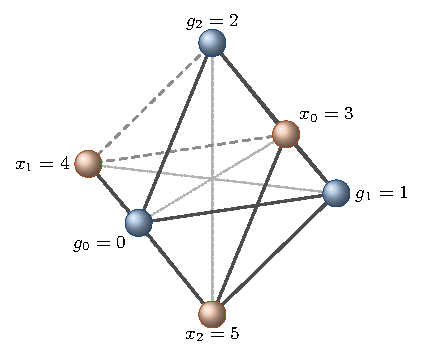
\includegraphics[width=0.42\textwidth]{figures/octahedron.pdf}
\caption{The octahedron $\oct$. Each vertex is adjacent to all others except its antipode; the dotted segments join the antipodal pairs $\{g_t,x_t\}$.}\label{fig:oct}
\end{figure}

\begin{lemma}\label{lem:oct}
$\ggr(\oct)=2$.
\end{lemma}

\begin{proof}
The sequence $(g_0,x_0)$ is legal: $x_0$ footprints itself. Conversely, let $(u,v)$ be legal. If $v$ is the antipode of $u$, then $N[u]\cup N[v]$ is the whole vertex set; otherwise $N[u]$ misses only the antipode of $u$, which lies in $N[v]$. Either way nothing is left for a third vertex to footprint.
\end{proof}

In $H_N$ we write $a_i=3i$, $b_i=3i+1$ and $c_i=3i+2$. Two vertices of the same residue class are never adjacent, and for vertices of different classes,
\begin{equation}\label{eq:adj}
  a_i\sim c_j\iff j\ge i,\qquad b_i\sim a_j\iff j>i,\qquad c_i\sim b_j\iff j>i,
\end{equation}
because $c_j-a_i=3(j-i)+2$, $a_j-b_i=3(j-i)-1$ and $b_j-c_i=3(j-i)-1$.

\section{A long legal sequence in the product}\label{sec:product}

The construction uses one property of $H_N$: with the colouring $v\mapsto v\bmod 3$, every edge $uv$ with $u<v$ satisfies $u\equiv v+1\pmod 3$. We state it for any graph with this property.

\begin{proposition}\label{prop:product}
Let $H$ be a graph with vertices $v_0,\dots,v_{N-1}$ and a map $t\colon V(H)\to\mathbb Z_3$ such that $t(v_i)\equiv t(v_j)+1\pmod3$ for every edge $v_iv_j$ with $i<j$. Then the sequence
\[
  s_j=\big(g_{t(v_j)},\,v_j\big),\qquad j=0,1,\dots,N-1,
\]
is legal in $\oct\sprod H$, and $\ggr(\oct\sprod H)\ge N$. In particular $\ggr(\oct\sprod H_N)\ge N$ for every $N\ge1$, with $t(v)=v\bmod3$.
\end{proposition}

\begin{proof}
We show that $s_j$ footprints $f_j=(x_{t(v_j)+1},v_j)$, indices of $g$ and $x$ taken modulo $3$. First, $f_j\in N[s_j]$: the vertex $x_{t(v_j)+1}$ is not the antipode $x_{t(v_j)}$ of $g_{t(v_j)}$, so it lies in $N[g_{t(v_j)}]$, and $v_j\in N[v_j]$. Now let $i<j$. If $f_j\in N[s_i]$, then $x_{t(v_j)+1}\in N[g_{t(v_i)}]$, which means $t(v_i)\ne t(v_j)+1$, and $v_j\in N[v_i]$, which for $i\neq j$ means that $v_iv_j$ is an edge, hence $t(v_i)=t(v_j)+1$. The two conclusions contradict each other, so $f_j\notin N[s_i]$.
\end{proof}

Figure~\ref{fig:product} shows the sequence for $H_{21}$. Every column of the product contains exactly one vertex of the sequence, while a Grundy dominating sequence of the form used for~\eqref{eq:lower} would use only $\ggr(H_{21})=10$ columns. The rotation of the three colours along the sequence is what lets each new vertex reach a footprint in a layer $x_t$ that none of the earlier vertices covers in that column.

\begin{figure}[ht]
\centering
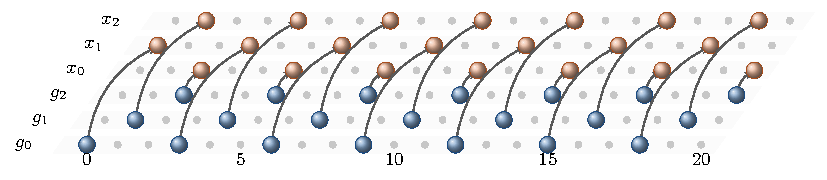
\includegraphics[width=\textwidth]{figures/product.pdf}
\caption{$\oct\sprod H_{21}$ as six stacked copies of $H_{21}$, one for each vertex of the octahedron. The $21$ blue vertices $(g_{j\bmod3},j)$ form a legal sequence; the arrow from each of them ends at its footprint $(x_{(j+1)\bmod 3},j)$.}\label{fig:product}
\end{figure}

\section{The family \texorpdfstring{$H_N$}{HN}}\label{sec:family}

We prove the formula for every $N\ge6$. A legal sequence in an induced subgraph remains legal in the larger graph, with the same footprints. We use this observation for both bounds.

\begin{lemma}\label{lem:upper-all}
For every integer $q\ge1$, $\ggr(H_{3q+1})\le q+3$.
\end{lemma}

\begin{proof}
Put $n=3q+1$. For $1\le d<n$, the conditions $d\equiv2\pmod3$ and $n-d\equiv2\pmod3$ are equivalent. Translation modulo $n$ therefore preserves adjacency. We may translate a nonempty legal sequence so that its first vertex is $0$.

This first vertex dominates $0$ and all the vertices $C_k=3k+2$, $0\le k<q$. The undominated vertices are
\[
 X_i=3(i+1),\qquad Y_j=3j+1\qquad(0\le i,j<q).
\]
There are no edges within either class, and
\begin{equation}\label{eq:half}
 X_i\sim Y_j\quad\Longleftrightarrow\quad i\ge j.
\end{equation}
Thus the remaining vertices induce a half graph with the perfect matching $X_iY_i$ (Figure~\ref{fig:half}).

\begin{figure}[tb]
\centering
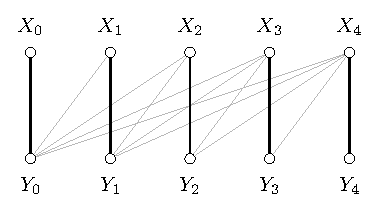
\includegraphics[width=0.85\textwidth]{figures/half-graph.pdf}
\caption{The undominated graph after selecting $0$ in $H_{3q+1}$, illustrated for $q=5$. The matching edges $X_iY_i$ are emphasized. Before the first selected edge, every selected $X$-index is smaller than every selected $Y$-index.}\label{fig:half}
\end{figure}


Follow the sequence until either a vertex $C_k$ is selected or the selected $X$- and $Y$-vertices contain an edge for the first time. Before either event, let $I,J$ be the selected indices on the two sides, and put $r=|I|$, $s=|J|$. Independence means
\begin{equation}\label{eq:independent}
 i<j\qquad(i\in I,\ j\in J).
\end{equation}

Suppose first that a new $X_i$ creates an edge. Then $J\ne\emptyset$ and $b=\min J\le i$. All earlier $X$-indices are less than $b$, so $i$ is the largest selected $X$-index. After this step, the undominated $X$-indices are $\{0,\dots,b-1\}\setminus I$, and the undominated $Y$-indices are those greater than $i$ that are not in $J$. Writing $s_0=|J\cap\{b,\dots,i\}|$, their total number is
\[
 b-r+(q-1-i)-(s-s_0).
\]
The number selected since $0$, plus the number still undominated, is
\[
 r+s+1+b-r+q-1-i-s+s_0=q+b-i+s_0\le q+1,
\]
because $s_0\le i-b+1$. Each later legal step must dominate a remaining vertex. The full sequence, including its initial $0$, has length at most $q+2$. If a new $Y$-vertex creates the first edge, use the same count after interchanging $X_i$ and $Y_{q-1-i}$; this interchange preserves~\eqref{eq:half}.

Suppose instead that $C_k$ is selected first. Its neighbours in the other two classes are the $X_i$ with $i<k$ and the $Y_j$ with $j>k$. Every vertex still undominated belongs to
\[
 W_k=\{X_i:k\le i<q\}\cup\{Y_j:0\le j\le k\},\qquad |W_k|=q+1.
\]
At least $r+s$ vertices in $W_k$ were already dominated. Indeed, map each earlier selection by
\[
 X_i\longmapsto\begin{cases}X_i,&i\ge k,\\Y_i,&i<k,\end{cases}
 \qquad
 Y_j\longmapsto\begin{cases}Y_j,&j\le k,\\X_j,&j>k.\end{cases}
\]
Each image is the selected vertex or its matching neighbour, so was already dominated. Images on each side are distinct. A collision between the sides would require an index in both $I$ and $J$, contrary to~\eqref{eq:independent}. The map is injective. At most $q+1-r-s$ vertices remain undominated, and the sequence has length at most
\[
 1+(r+s)+1+(q+1-r-s)=q+3.
\]

If neither event occurs, the vertices selected after $0$ form an independent set in the half graph. Its perfect matching bounds their number by $q$, so the full sequence has length at most $q+1$. These cases prove the lemma.
\end{proof}

\begin{lemma}\label{lem:lower-all}
If $N\ge6$ and $q=\lfloor(N+1)/3\rfloor$, then $\ggr(H_N)\ge q+3$.
\end{lemma}

\begin{proof}
For $q=2$, the sequence $(1,3,5,0,2)$ in $H_6$ has successive footprints $(1,5,0,2,4)$ and remains legal in $H_7$. For $q=3$, the sequence $(0,7,2,4,5,1)$ in $H_8$ has footprints $(0,7,4,6,3,1)$ and remains legal in $H_9$ and $H_{10}$.

For $q\ge4$, it suffices to work in $H_{3q-1}$, which is an induced subgraph of $H_N$. In the notation $a_i=3i$, $b_i=3i+1$, $c_i=3i+2$, take
\begin{equation}\label{eq:lower-sequence}
 a_0,a_1,\dots,a_{q-3},\ b_{q-1},\ c_{q-3},\ c_0,\ a_{q-2},\ b_0.
\end{equation}
The first $q-2$ vertices footprint themselves. The last five have successive footprints
\[
 b_{q-1},\quad b_{q-2},\quad b_{q-3},\quad a_{q-2},\quad a_{q-1}.
\]
By~\eqref{eq:adj}, $b_{q-1}$ is not adjacent to any earlier $a_i$; $b_{q-2}$ is first dominated by $c_{q-3}$; and $b_{q-3}$ is first dominated by $c_0$. Here $q-3>0$, so $c_0\sim b_{q-3}$. Neither $a_{q-2}$ nor $a_{q-1}$ is adjacent to $b_{q-1}$, $c_{q-3}$ or $c_0$. Thus $a_{q-2}$ footprints itself, and $b_0$ footprints $a_{q-1}$. The sequence has length $q+3$.
\end{proof}

\begin{proof}[Proof of Theorem~\ref{thm:family}]
Put $q=\lfloor(N+1)/3\rfloor$. Since $N\le3q+1$, the graph $H_N$ is an induced subgraph of $H_{3q+1}$. Lemma~\ref{lem:upper-all} gives the upper bound $q+3$, and Lemma~\ref{lem:lower-all} gives equality. The product bound is Proposition~\ref{prop:product}.

At $N=19$ the formula gives $\ggr(H_{19})=9$. For $N\ge21$, write $N=3q-1$, $3q$ or $3q+1$. The respective differences $N-2(q+3)$ are $q-7$, $q-6$ and $q-5$. Each is positive in its applicable range. Hence $N>2\ggr(H_N)$ for $N=19$ and every $N\ge21$.
\end{proof}


\section{Further questions}
\begin{question}
Which graphs $G$ satisfy Conjecture~\ref{conj} for every $H$? All forests do~\cite{BDKW}, whereas the octahedron does not.
\end{question}

\appendix
\section{The finite certificate for \texorpdfstring{$H_{21}$}{H21}}\label{sec:H21}

\begin{lemma}\label{lem:h21lower}
$\ggr(H_{21})\ge10$.
\end{lemma}

\begin{proof}
The sequence
\[
 \begin{aligned}
 &(a_0,a_1,a_2,a_3,a_4,b_6,c_4,c_0,a_5,b_0)\\
 &\qquad=(0,3,6,9,12,19,14,2,15,1)
 \end{aligned}
\]
is legal and dominating. By~\eqref{eq:adj}, $a_0$ dominates $c_0,\dots,c_6$; each $a_i$ with $1\le i\le4$ footprints itself and $b_{i-1}$; then $b_6$ footprints itself, $c_4$ footprints $b_5$, $c_0$ footprints $b_4$, $a_5$ footprints itself and $b_0$ footprints $a_6$.
\end{proof}

Theorem~\ref{thm:family} already proves the upper bound without a computer. For an independent finite certificate we use the sets of dominated vertices. For a legal sequence $S=(v_1,\dots,v_k)$ put $D(S)=N[v_1]\cup\dots\cup N[v_k]$. Define families $\mathcal L_0,\mathcal L_1,\dots$ of vertex sets by $\mathcal L_0=\{\emptyset\}$ and
\[
  \mathcal L_{k+1}=\big\{\,D\cup N[v]\;:\;D\in\mathcal L_k,\ v\in V(G),\ N[v]\not\subseteq D\,\big\}.
\]

\begin{lemma}\label{lem:layers}
If $S$ is a legal sequence of length $k$, then $D(S)\in\mathcal L_k$. Hence $\ggr(G)$ is the largest $k$ with $\mathcal L_k\neq\emptyset$.
\end{lemma}

\begin{proof}
Induction on $k$: if $(v_1,\dots,v_{k+1})$ is legal, then $D=D(v_1,\dots,v_k)\in\mathcal L_k$ and $N[v_{k+1}]\not\subseteq D$, so $D\cup N[v_{k+1}]\in\mathcal L_{k+1}$. Conversely, every member of $\mathcal L_k$ is $D(S)$ for a legal sequence $S$ of length $k$, by the same induction.
\end{proof}

The families can be large in general, but for $H_{21}$ they are small: by~\eqref{eq:adj}, the vertices of a class dominated by the vertices of another class form an initial or a final segment of that class.\footnote{For instance, the vertices $c_j$ dominated by the chosen vertices of the class $a$ are those with $j\ge\min\{i: a_i\text{ chosen}\}$.} Their sizes are
\[
  |\mathcal L_0|,\dots,|\mathcal L_{10}| = 1,\ 21,\ 210,\ 1023,\ 1482,\ 1302,\ 848,\ 419,\ 150,\ 22,\ 1,
\]
and $\mathcal L_{11}=\emptyset$; the only member of $\mathcal L_{10}$ is the whole vertex set. With Lemma~\ref{lem:layers} this gives the following.

\begin{proposition}\label{prop:h21upper}
$\ggr(H_{21})\le10$.
\end{proposition}

We have verified Proposition~\ref{prop:h21upper} in three independent ways. In Lean~4, a certificate lists the $5479$ sets of the families $\mathcal L_0,\dots,\mathcal L_{10}$ as bit masks stored in binary search trees, and the kernel checks by evaluation that $\emptyset\in\mathcal L_0$, that $D\cup N[v]\in\mathcal L_{k+1}$ for every $D\in\mathcal L_k$ and every $v$ with $N[v]\not\subseteq D$, and that no member of $\mathcal L_{10}$ has a proper extension. A formal version of Lemma~\ref{lem:layers}, proved in Lean for every graph and every such certificate, then bounds the length of every legal sequence of $H_{21}$ by $10$. The formal counterexample uses the definitions in this paper and only standard axioms; no \texttt{native\_decide} is used. Independently, a C program computes the families by breadth-first search, and a Python program finds $\ggr(H_{21})=10$ by a memoised depth-first search over dominated sets; both use only the definition of $H_{21}$.

\begin{corollary}\label{thm:main}
$\ggr(\oct)=2$, $\ggr(H_{21})=10$, and
$\ggr(\oct\sprod H_{21})\ge21>2\cdot10$.
\end{corollary}
\begin{proof}
Lemma~\ref{lem:oct}, Theorem~\ref{thm:family} at $N=21$, and Proposition~\ref{prop:product} prove the result. Lemma~\ref{lem:h21lower} and Proposition~\ref{prop:h21upper} give the separate finite verification.
\end{proof}


\subsection*{Computations and formal verification}
The repository~\cite{Revision} contains the Lean development, the Python and C programs, build commands and current verification results. The archived original development is~\cite{Ar}. Lean~4~\cite{MU} is pinned to version~4.34.1 and this development needs no external Lean library. The Lean certificate concerns only $N=21$. Neither the all-$N$ formula nor the unbounded-ratio theorem has been formalized. Both have complete written proofs above. Finite checks accompany them without replacing those proofs.

\subsection*{Use of generative AI}
Claude (Anthropic) assisted with the original computations, Lean development and drafting. ChatGPT (OpenAI) assisted the exact-support rank argument and two-field construction in Section~\ref{sec:unbounded}, using Alon's method as identified there; it also assisted the all-parameter half-graph count and explicit footprints in Section~\ref{sec:family}. OpenAI Codex assisted this revision with proof auditing, checks, organization, bibliography and typesetting. The human author is responsible for the correctness of the manuscript and its citations.

\bibliographystyle{aomplain}
\bibliography{references}
\end{document}
